\documentclass{beamer}
\usepackage{color}% or package color
\usepackage{cancel}
\usepackage{amsmath}
\usepackage{amsfonts}
\usepackage{amssymb}
\usepackage{cases}
\usepackage{animate}
\usepackage{tikz}


\renewcommand{\thefootnote}{\fnsymbol{footnote}}

\newcommand{\laplinv}{\mathcal{L}^{-1}}
\newcommand{\eF}{e^{-i \xi x }}
\usepackage{xmpmulti} % animations

\renewcommand{\epsilon}{\varepsilon}

\usetheme{Madrid}


\title{Optimized Schwarz Method for the Linearized KdV equation and for coupling a NSWE-Serre model}

\author{J. Caldas \inst{1}
	 \and R. Cienfuegos \inst{3}
	 \and \textbf{J. Galaz}  \inst{3}
	 \and A. Rousseau \inst{2}
}

\institute[PUC+Meric] % (optional, but mostly needed)
{
  \inst{1}%
  MERIC, Chile
  \and
  \inst{2}%
  Inria and Inria Chile
  \and
  \inst{3}%
  Department of Hydraulic and Environmental Engineering, Pontifical Catholic University of Chile
}

 
\date{WTE2016}
\begin{document}
  \begin{frame}
    \titlepage
  \end{frame}

  \section{Introduction}
  \begin{frame}{RL1.6 on Resource Assesment and Site Characerization}{Advanced modelling for marine energy}
  
  \vspace{-0.5cm}
  \begin{center}
    \includegraphics[width=0.7\textwidth]<1>{figures/figmodels/Diapositiva1.PNG}
    \includegraphics[width=0.7\textwidth]<2>{figures/figmodels/Diapositiva2.PNG}
    \includegraphics[width=0.7\textwidth]<3>{figures/figmodels/Diapositiva3.PNG}
    \includegraphics[width=0.7\textwidth]<4->{figures/figmodels/Diapositiva4.PNG}
  \end{center}
    
    \begin{block}{Question}<4>
      Can we make these different models \alert{communicate} with each other?
    \end{block}
    
    % \begin{block}{Remark}
    %   Self-coupling can be used with complex geometries and for parallelization
    % \end{block}    
  \end{frame}


  \begin{frame}{Truncated domain error: A tsunami simulation}{Nonlinear long wave model (GeoClaw from the U. Washington)}
    \begin{center}
    \begin{tikzpicture}
      \node<1-2> (img1) at (-2,0) {\animategraphics[loop,width=0.4\linewidth]{1}{figures/bigdomain/fr-}{1}{5}};
      \pause
      \node<2> (img2) at (2,0) {\animategraphics[loop,width=0.3\linewidth]{1}{figures/smalldomain/fr-}{1}{5} };
      \pause
      \node<3-> (img3) at (0,0) {\animategraphics[loop,width=0.5\linewidth]{12}{figures/erroranimation/error-}{1}{39} };
    \end{tikzpicture}
    \end{center}


    \begin{block}{Challenges}


      \begin{itemize}
        \item Long simulations are required for statistics estimates
        \item Transport of the numerical error from deep to shallow water: shoaling
      \end{itemize}
    \end{block}
  \end{frame}

  \begin{frame}{Our work}
    \begin{block}{First results }
      \begin{itemize}
        \item Develop a self coupling methodology: Domain Decomposition Methods (DDM)
        \pause

        \item Study the most fundamental equation for \textcolor{red}{non-linear} and \textcolor{blue}{dispersive} waves: The KdV equation
        $$ u_t + u_x + \textcolor{red}{uu_x}+ \textcolor{blue}{u_{xxx}} = 0$$
        \pause

        \item Simplify even more: keep only the \textcolor{blue}{dispersive} part
        $$ u_t + \textcolor{blue}{u_{xxx}} = 0$$
      \end{itemize}
    \end{block}

    \pause
    \begin{block}{Ongoing work}
      Develop a coupled model between the  \textcolor{red}{Non Linear Shallow Water Equations} (NSWE) and the \textcolor{blue}{Serre equations}
    \end{block}
  \end{frame}

  \section{DDM for the KdV equation}
  \subsection{Intuition}
    \begin{frame}{A key ingredient: \emph{Transparent} Boundary Conditions (TBC)}
      \begin{columns}
        \column{0.5\textwidth}
            \includegraphics[width=\textwidth]<1-2>{figures/TBCs/Diapositiva1.PNG}
            \includegraphics[width=\textwidth]<3>{figures/TBCs/Diapositiva2.PNG}
            \includegraphics[width=\textwidth]<4>{figures/TBCs/Diapositiva3.PNG}
            \includegraphics[width=\textwidth]<5->{figures/TBCs/Diapositiva4.PNG}
        \column{0.5\textwidth}
          \begin{enumerate}
            \item<1->  Start with an infinite domain: 
            \item<2->  Seek for an exact explicit solution  \alert{$\hdots$ and fail} (most of the time) 
            \item<3->  \alert{Truncate} the domain: approximate numerical solution 
            \item<4->  \emph{Apply} Laplace transform to the equation at the boundaries of the \alert{infinite domain} (unknown), formulate candidate solutions  
            \item<5->  \textit{Un-apply} it and get new equations for the boundaries
          \end{enumerate}
      \end{columns}

    \end{frame}

    \begin{frame}{Transparent Boundary Conditions (TBC's)}
      \begin{block}{Exact TBC's (Besse et al, 2015)}
        \begin{itemize}
          \pause
          \item Solving these equations is also \alert{\emph{very}} hard (non-local operator)
            \begin{equation*}
              \begin{cases}
                      u(t,\textcolor{blue}{left}) - \alert{\laplinv} \left( \frac{\lambda_1(s)^2}{s} \right) \alert{*} u_x(t,a) - \alert{\laplinv} \left( \frac{\lambda_1(s)}{s} \right) \alert{*} u_{xx}(t,a) = 0 \\
                      u(t,\textcolor{blue}{right}) - \alert{\laplinv} \left( \frac{1}{\lambda_1(s)^2} \right) \alert{*} u_{xx}(t,b) = 0 \\
                      u_x(t,\textcolor{blue}{right}) - \alert{\laplinv} \left( \frac{1}{\lambda_1(s)} \right) \alert{*} u_{xx}(t,b) = 0
              \end{cases}
            \end{equation*}
            \pause
          \item Not suited for numerical computations!
        \end{itemize}
      \end{block}

    \end{frame}

    \begin{frame}{Approximate TBC's}
      \begin{block}{Result}
        Using the approximation $\lambda(s) \approx c$ we obtain the following approximate TBC's
        \begin{equation*}
            \begin{cases}
                u(t,\textcolor{blue}{left}) - c u_x(t,\textcolor{blue}{left})  + c^2  u_{xx}(t,\textcolor{blue}{left}) = 0 \\
                u(t,\textcolor{blue}{right}) - c^2    u_{xx}(t,\textcolor{blue}{right}) = 0 \\
                u_x(t,\textcolor{blue}{right}) + c u_{xx}(t,\textcolor{blue}{right})= 0
            \end{cases}
        \end{equation*}
      \end{block}

    \end{frame}

    \begin{frame}{Using the TBC's for a DDM: The Additive Schwarz Method}
        \begin{center}
            \includegraphics[height=0.4\textheight]<1>{figures/ddm/Diapositiva1.PNG}
            \includegraphics[height=0.4\textheight]<2>{figures/ddm/Diapositiva2.PNG}
            \includegraphics[height=0.4\textheight]<3>{figures/ddm/Diapositiva3.PNG}
            \includegraphics[height=0.4\textheight]<4->{figures/ddm/Diapositiva4.PNG}
        \end{center}
        
      
      \begin{block}{DDM Methodology}
        \begin{itemize}
          \item<2->  Solve each problem separately, using the adjacent domain last information.
          \item<3-> Iterate until convergence criteria.
          \item<4-> How do we determine the $c_L$ and $c_R$ constants ?
        \end{itemize}
      \end{block}
    \end{frame}

    \begin{frame}{DDM: Determination of optimal $c_L=c_R = c$}
      \begin{itemize}
        \item For a fixed mesh discretization (in time and space), fixed interface location and different  time-steps (initial condtion)
      \end{itemize}
        
        \begin{center}
            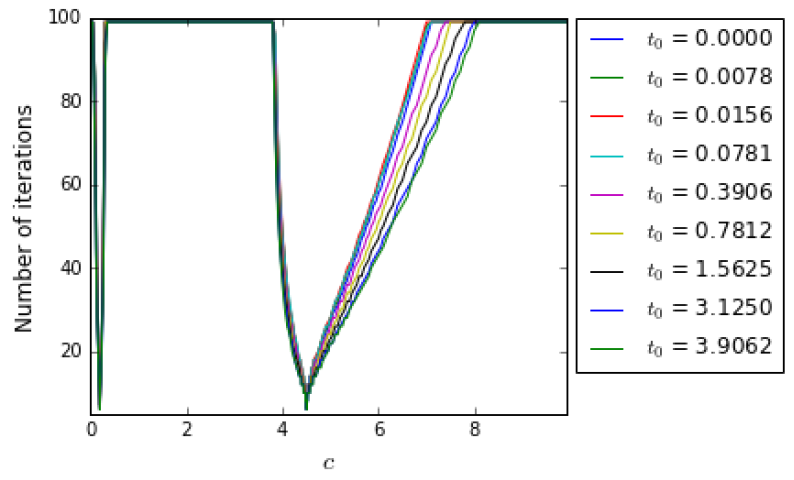
\includegraphics[width=0.5\textwidth]{figures/results/c_vs_it_formanyt0.PNG}
        \end{center}
        \pause
      \begin{block}{Remark}
        \begin{itemize}
          \item There exist \textcolor{blue}{optimal values} for $c$ (e.g $\approx 4.5$) where convergence is observed with (only) 5-7 iterations.
          \pause
          \item There is no observed dependency on the \textcolor{blue}{initial condition}.
        \end{itemize}
      \end{block}

    \end{frame}

    \begin{frame}{DDM: Dependency on the location of the interface}
      \begin{center}
        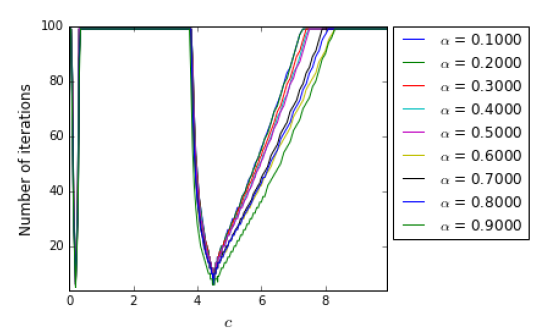
\includegraphics[width=0.5\textwidth]{figures/results/c_vs_it_interface.PNG}
      \end{center}
      
      \begin{block}{Remark}
        There is no observed dependency on the location of the interface
      \end{block}
    \end{frame}

    \begin{frame}{DDM: Dependency on the discretization size: $\Delta x$, $\Delta t$}
      \begin{center}
        \includegraphics[height=0.4\textheight]<1>{figures/results/c_vs_it_dxdt.PNG}
        \includegraphics[height=0.4\textheight]<2->{figures/results/copt_dxdt.PNG}
      \end{center}

      \pause
      \begin{block}{Result}
        There is a strong dependance on $\Delta x$ and $\Delta t$. \pause Furthermore the regression
        $$ c_{opt}(\Delta t, \Delta x)  = \kappa + \alpha (\Delta t)^{2/3} + \beta \frac{1}{\Delta x} + \gamma \frac{\Delta t^{2/3}}{\Delta x}$$

        fits the numerical experiments with
        $R^2 = 0.9999894$ \pause for
        $\kappa = 0.0775$,
        $\alpha = -0.3353$,
        $\beta = -0.0012$,
        $\gamma = 2.7407$
      \end{block}
    \end{frame}

  \section{Coupled NSWE-Serre model}

  \begin{frame}{A coupled shallow water (NSWE) - Serre model}
    \begin{block}{The Serre equations}
      \begin{equation*}
        \begin{split}
          h_t + (hu)_x = 0 \\
          u_t + uu_x + gh_x - \textcolor{blue}{\frac{1}{3h}\left(h^3 \left( u_{xt} + uu_{xx} - (u_x)^2  \right) \right)_x} = 0
        \end{split}
      \end{equation*}
        \begin{itemize}
            \item $h=$ the water column height
            \item $u=$ depth averaged horizontal velocity (1D)
        \end{itemize}      
    \end{block}
  \end{frame}

  \begin{frame}{Coupling methodology}
  \begin{center}
  \includegraphics[height=0.9\textheight]<1>{figures/serrenswe/Diapositiva1.PNG}
  \includegraphics[height=0.9\textheight]<2>{figures/serrenswe/Diapositiva2.PNG}
  \end{center}
    \begin{block}<3->{Numerical method}
        \begin{itemize}
            \item Fractional splitting scheme for non-linear/dispersive terms (Bonneton et al, 2011).
            \item Well-balanced fourth order accurate Finite Volume NSWE model (Berthon and Marche,2008)
            \item Fourth order Finite Difference model for the dispersive equation
        \end{itemize}
    \end{block}
      
  \end{frame}
  
  \begin{frame}{Three domain coupling: NSWE-Serre-NSWE}
    \begin{center}
        \animategraphics[loop,width=0.8\linewidth]{10}{figures/threedomains/threedomains-}{1}{29}
    \end{center}      
  \end{frame}
\end{document}
